\documentclass[12pt,letter]{article}
\usepackage{amssymb,microtype,tikz, amsmath, hyperref,setspace,todonotes}
\usepackage[T1]{fontenc}
\usepackage{color,parskip,siunitx,physics,marginnote}
\DeclareMathAlphabet{\mathscr}{OT1}{pzc}{m}{it}
\usepackage{epsfig, graphicx,subcaption,caption}
\usepackage{verbatim,marginfix}
\captionsetup[widefigure]{size = \textwidth}
%\renewcommand{\footnotesize}{\scriptsize}
%\usepackage{mparhack}
\usepackage[letterpaper, driver=xetex,inner=2cm, outer=7cm, marginparsep=.5cm,
    marginparwidth=6cm, 
twoside=true]{geometry}
\usepackage[maxfloats=45]{morefloats}
\newcommand{\marginparstyle}{\footnotesize} % initialize style with start value
  \renewcommand*{\marginfont}{\marginparstyle}
\let\oldmarginpar\marginpar
\renewcommand*{\marginpar}[1]{\oldmarginpar{\begin{singlespace*} \marginparstyle #1
\end{singlespace*}}}
%\usepackage{ebgaramond}
\usetikzlibrary{shapes.geometric, arrows}
\usepackage{sidenotes}
\usepackage{booktabs,adjustbox,authblk}
\title{Laser-Wakefield Electron Accelerators}
\author{Adam A. S. Green}
\affil{\small Department of Physics, University of Colorado at Boulder}
\begin{document}
\bibliographystyle{abbrv}
\maketitle
\doublespacing
\strictpagecheck
\begin{abstract}
    In the late 1970's, Tajima and Dawson published a seminal paper in {\em
    Physical Review Letters} outlining a new kind of electron
    accelerator that was orders of magnitude smaller than conventional
    technology. It
    worked by
    leveraging the high-energy gradients of
    laser-excited plasmas to accelerate electrons over centimeter length scales to \si{\giga\electronvolt}
    energies. Their proposal was untenable at the time as it
    required lasers with peak intensities far beyond the technology of the era.
    It has only been recently, through a combination of modern laser technology and powerful new
    numerical methods, that researchers have been able to make dramatic
    progress in the field. Several groups are now poised to deliver on the
 original promise of Tajima and Dawson.
    
    In this work, we review the field of Laser Wakefield Plasma Accelerators
    (LWPA) covering the historical beginnings, the physical underpinnings,
    and close with a discussion of current state-of-the-art
    experimental results. 

  \end{abstract}
\tableofcontents
\section{Introduction}
\label{sec:intro}
Conventional methods of electron acceleration use a TM-mode rf field
propagating in a
waveguide to provide the acceleration gradient. Waveguide field gradients are
fundamentally limited by electric breakdown on the walls of the waveguide to
approximately a
\si{\mega\electronvolt\per\meter}\cite{wang1997field}. This means that to achieve the
\SI{50}{\giga\electronvolt} energies currently used at the Stanford Linear
Accelerator Center
(SLAC)\cite{cornacchia2000coherent}, the waveguide has to be about 2 miles long. In contrast, the
acceleration gradients in plasmas can easily exceed \SI{10}{\giga
\electronvolt\per\meter}, thereby allowing electrons to be accelerated over centimeters
for similar energy gains\cite{RevModPhys.81.1229}.
The study of LWPA is strongly motivated by this promise of table-top electron
accelerators.   

 
 The broadest application of high-energy electrons today is their use in
 free-electron x-ray lasers. The development of
 which has allowed investigation of structures in biology, solid state
 physics, as well as pioneering techniques in medical
 imaging\cite{o2001free,pellegrini2003x}.
 Currently, free-electron x-ray lasers are tied to the large linear accelerators that provide them
 with electrons. LWPA offers a smaller low-cost platform for electron
 acceleration, which would allow a broader use of x-ray lasers in the
 scientific community.  The dissemination of more economical x-ray
 lasers would not only encourage more research but would also reduce the risk of
 limiting research due to damage or funding cuts to the larger, high-cost
 facilities\sidenote{The famous cancellation of the Superconducting Super
 Collider in Texas due to budget problems in one dramatic example.}. Much like the impact of personal
 computers introduced in the era of massive supercomputers, the impact of a
 small cheap x-ray laser  will be dramatic\cite{mcneil2010x}. 


 The goal of LWPA technology is to produce
 a large number of high-energy electrons with a narrow energy distribution in a collimated beam.
It is an exciting
 time for LWPA as it is only
 within the past decade that LWPA technology became capable of meeting the above
 requirements. 
 \subsection{History}
 \label{sec:history}
Tajima and Dawson originally proposed shooting a high-intensity laser pulse at a
 plasma\cite{PhysRevLett.43.267}. The photon-pressure of the laser
 generated a wakefield and electrons could `surf' this wake and be accelerated.
  Unfortunately, the lasers of the day could not reach the high intensities
  required. It was the invention of 
 chirped-pulse amplification (CPA) and resulting high-intensity lasers that
 allowed serious progress in
 the LWPA field to occur\cite{backus1998high}.
\begin{marginfigure}
	\includegraphics[width=\marginparwidth]{../figures/datfig.pdf}
    \caption{\label{fig:progress}The progress of laser plasma wakefield acceleration by the total
    energy of the electrons. The dashed line shows the advent of
    quasi-monoenergetic electrons, until that point the electron bunches had
    large thermal tails. \em This data was gathered from the Web of Science
abstract search tool.}
\end{marginfigure}Even when the intensity issue had been overcome there were
still severe experimental constraints, as exciting the plasma wave
requires the laser duration to be at $\tau_\textrm{duration} \approx
1/\omega_p$, where $\omega_p$ is the natural plasma frequency which scales with the square-root of the plasma density. For typical
laboratory plasmas, $\tau_\textrm{duration}$ was out of reach for the lasers of
the time. To overcome this problem several LWPA schemes were devised; the two major ones being the plasma beatwave accelerator and the
self-modulated laser accelerator\cite{RevModPhys.81.1229}. Although the mechanics of these schemes
differed, the
underlying principle was to excite the plasma with a beatwave generated by spatio-temporally
overlapping two lasers detuned from each other by $2\pi\omega_p$. It would
require further refinement of laser technology before lasers could directly
excite the plasma. Unfortunately, the electron beams generated using these
schemes all had broad
Maxwellian energy distributions, making them unsuitable for practical
applications requiring mono-energetic electrons.

 A breakthrough occurred in 2002, when Pukhov
 predicted the bubble regime in
 simulation\cite{pukhov2002laser}. The bubble regime would solve many of the
 problems faced by LPWA schemes and is so
 named as it uses a laser powerful enough to
 completely expel electrons from the pulse region, creating an ion `bubble'. One
 of the most attractive properties of the bubble regime was its predicted ability to
 produce mono-energetic electrons. 

 In 2004, this approach bore fruit as three papers, published simultaneously in
 Nature\cite{mangles2004monoenergetic,faure2004laser,Geddes2004}, demonstrated
 quasi-monoenergetic electron bunches in the bubble regime. In 2006, their results were
 extended to achieve energies of \SI{1}{\giga\electronvolt}
 \cite{Leemans2006}. 
 
 In 2013, a group at UT Austin produced a collimated, quasi-monoenergetic
 electron beam at 2.3 GeV\cite{Wang2013}, and in 2014, the Esarey group at UC
 Berkeley produced a 4 GeV\cite{PhysRevLett.113.245002} beam. These recent
 developments bring the field within striking distance of the LCLS free electron
 laser at SLAC,
 which uses electrons accelerated to \SI{17.4}{\giga\electronvolt}\cite{cornacchia2000coherent}.

\section{The Physics of Laser-Plasma-Acceleration}
\begin{marginfigure}
    \resizebox{.9\textwidth}{!}{
    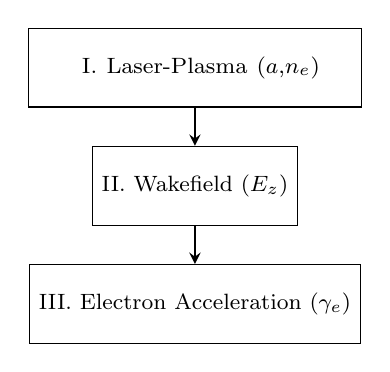
\begin{tikzpicture}[scale =.5,node distance = 1.5cm,auto]
        \node[draw,rectangle,minimum height=1cm,minimum width=2cm,text
        centered, text width = 4 cm,name=input]
        {\footnotesize \setstretch{1} I. Laser-Plasma ($a$,$n_e$)\\};
        \node[draw, rectangle, text centered, minimum height=1cm, minimum
        width=2cm, below of=input] (wakefield) {\footnotesize II. Wakefield ($E_z$)};
        \node[draw, rectangle, minimum height=1cm, text centered, minimum
        width=2cm, below of=wakefield] (eaccel) {\footnotesize III. Electron
        Acceleration ($\gamma_e$)};
        \draw  [thick,->,>=stealth] (input) -- (wakefield);
        \draw  [thick,->,>=stealth] (wakefield) -- (eaccel);
    \end{tikzpicture}
}
\caption{\label{fig:flow}The LWFA process. }
\end{marginfigure}
   
The LPWA process is divided into three main segments as shown in Figure
\ref{fig:flow}. First the intense laser, characterized
by the normalized field strength $a = eA/m_e c^2$, with $A$ as the laser vector
potential, interacts with the
plasma, characterized by the plasma density $n_e$. This then produces a longitudinal
density modulation, which in turn gives rise to a longitudinal electric
wakefield, $E_z$. The wakefield then accelerates injected electrons to a relativistic energy
$\gamma_e$. This section reviews these three inter-related phenomena\sidenote{Due to the complicated nature of the theory of LPWA in 3D relativistic fields, we will mainly
discuss these topics in the linear regime and show the numerical results of
their extension into the 3D relativistic regime.}. 
\subsection{The Laser-Plasma Interaction and Creation of Wakefields}
\label{sec:wakefield}
The mass of the ions in the plasma is many orders of magnitude larger than the
electrons, so it is valid to approximate the plasma as a fluid of
mobile electrons against a static background of ions. The motion of the
electrons is then governed by the
combination of the Lorentz force, the continuity equation, and Poisson's
equation. Additionally, if the
intensity of the laser is small enough ($a\ll 1$), then these equations can be
linearized and are referred to as the cold-fluid
equations\cite{gorbunov1987excitation}.
In the cold-fluid regime, the Lorentz force takes the following form:
\begin{align}
    \label{eq:fullLPWA}
    \pdv{\vb{p}}{t} +(\vb{v} \cdot \grad)\vb{p} = e \qty(
    \pdv{\vb{A}}{t} - \vb{v}\times \grad \times \vb{A} )
\end{align}

Where $\vb{p}$, $\vb{v}$ are the electron's momentum and velocity, 
and $\vb{A}$ is the vector potential of the field.

The linear behaviour of this fluid will be dominated by the force of the
electric field on the electrons, accelerating them in the polarization
plane. This is called the `quiver' momentum\sidenote{So named because the electron will
undergo rapid oscillations while its time averaged acceleration will be zero, so it will appear to be quivering}. Considering the next leading order behaviour of the electron momentum and
averaging over one
optical cycle, we get a force that is proportional to the intensity gradient of the laser pulse. This is known as the
ponderomotive force\cite{RevModPhys.81.1229} and can be
thought of as the radiation pressure of the laser pulse pushing
electrons away from its local space. As the laser propagates
through the plasma the ponderomotive force will drive a density wave known as a
plasmon, analogous to the physical situation of shooting a
cannonball underwater.

The solution for the density fluctuations in the cold-fluid
regime is given by\cite{RevModPhys.81.1229}:
\begin{equation}
    \label{eq:wave}
    \qty( \pdv[2]{t} + \omega_p^2 )\delta_{n_e} = c^2 \laplacian \frac{a^2}{2}
\end{equation}
where $a$ is the normalized vector potential, $\delta_{n_e}$ is the density
fluctuation
of the electron fluid and $\omega_p$ is the plasma frequency.

Connecting the density fluctuations to
the electric field produced using Possion's equation under the assumption
of periodic behaviour in $\vb{E_z}$ results in the wakefield equation:
\begin{equation}
    \vb{k}\dotproduct\vb{E_z} = \frac{\delta n_e}{\epsilon_0}
\end{equation}

Showing that an electric field oriented along the propagation axis will
co-propagate $\pi$ out of phase
with the plasmon. We show this in the linear
and non-linear 1D regime in Figure \ref{fig:plasmon1}. $E_z$ will be the accelerating field that LWPA uses.

\begin{marginfigure}[0pt]
    \includegraphics[width=\marginparwidth]{../figures/esblowout.pdf}
    \caption{\label{fig:bubble} An example of the bubble regime created by a laser pulse with $a =
    .3$. The laser is moving toward the right, and $\delta_n =\frac{n}{n_0}$,
with $n$ being the density of the electrons and $n_0$ being the density of the
ions. The coordinates are dimensionaless and show the evolution of the
phase-front.\cite{RevModPhys.81.1229}}
\end{marginfigure}


All modern LWPA approaches operate in the
bubble regime so we must extend our linear 1D model to a highly
non-linear  2D or 3D model. We can access this regime by relaxing 
the assumption that $a \ll 1$ and an analytical solution in 1D can still be
found\cite{sprangle1990nonlinear}. However, in 2D or 3D, the equations become intractable and numerical simulation is
required. An example of a numerical solution in a non-linear 2D model is shown
in Figure \ref{fig:plasmon2}, and an example of the bubble regime is shown in
Figure \ref{fig:bubble}.

\begin{figure}[h!]
        \begin{singlespace*}
        \centering
        \label{fig:plasmon}
        \begin{subfigure}[t]{\textwidth}
            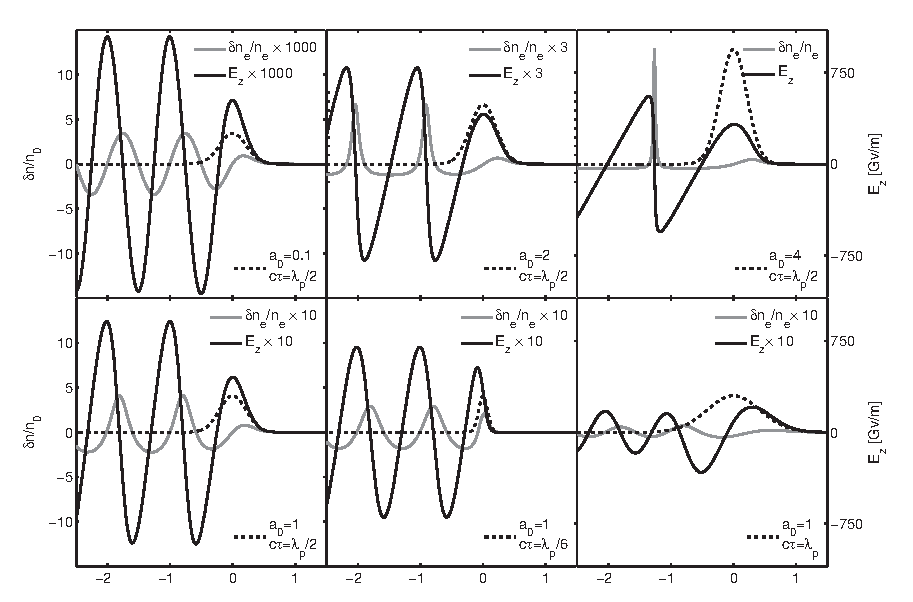
\includegraphics[height = .35\textheight]{../figures/densityandewave.eps}
            \caption{\small  Showing plasmons generated with varying strengths of the peak
                amplitude of the laser pulse.\cite{genothesis}\label{fig:plasmon}
                The laser pulse is the dashed line, the density perturbation is the grey
                line, and the longitudinal electric field $E_z$ is the black
                curve. The x-axis is showing the normalized co-ordinate $\xi =
                kz - wt$, which shows the evolution of the phase-front. Different
                scenarios are shown: from left to right, the normalized field strength variable
                ($a = eA/m_e c^2$) is varied, and from top to bottom, the duration of
            the laser pulse is changed.}            \label{fig:plasmon1}
        \end{subfigure}

        \begin{subfigure}[t]{\textwidth}
            \includegraphics[height = .3\textheight]{../figures/esarey3dnonlin.pdf}

            \caption{\small  Numerical simulation for a 2D, non-linear model. Many of the
                features in the 1D model remain-- the signature `leaning' of the density
                pulse as it becomes non-linear being the most
            striking.\cite{RevModPhys.81.1229} }
            \label{fig:plasmon2}
        \end{subfigure}
        \caption{\small Plasmons in 1 and 2 dimensions.}
\end{singlespace*}
    \end{figure}
   \subsection{Electron Dynamics}
   Before we can review how electrons are
    accelerated, we first must discuss how they are trapped in the wakefield.    \subsubsection{Trapping Electrons}
    In Figure \ref{fig:plasmon} we mentioned that electrons need
    to be injected into the wakefield. Because the wakefield will be
    co-propogating with laser pulse --moving close to the speed of light-- a
    stationary electron in the lab frame won't interact with it long enough to
    be accelerated.
    To illustrate the point, several phase-space trajectories of test electrons
    with various initial momenta are shown in Figure
    \ref{fig:trapping}. Some minimum electron velocity is required and this can
    either be achieved by externally injecting electrons, or by taking
    advantage of the non-linear processes in the bubble regime to self-inject
    electrons from the surrounding fluid\sidenote{Interesting,
    although self-injection happens in
        non-linear fields in both 1D and 3D, it occurs by different physical
    processes\cite{esatrap}. We will be focusing on the 3D case in this
review.}.
\begin{figure}[h!]%
    \includegraphics[width=\textwidth]{../figures/trapping.pdf}
    \caption{\label{fig:trapping} The various trajectories of electrons at
    different initial normalized momentum ($u_z= p/m_e c^2$) in the reference frame of the laser
pulse, which is moving at an relativistic energy $\gamma = 13$ in the lab frame.
An electron injected at the phase-space point \textbf{a} will be trapped, and
accelerated by the wakefield through point \textbf{c} until it gains its maximum
momentum at point \textbf{c}. At point \textbf{c}, it will be `dephased' as it has overtaken
the accelerating wakefield, at which point it drops back to point \textbf{a}. An
experiment has to be designed so that the electrons are harvested at the
dephasing point \textbf{c}. The black curve is the seprratric, which seperates
trapped electrons from untrapped electrons. $\xi$ is the normalized
co-ordinate showing the phase-front evolution\cite{genothesis}.}

\end{figure}
    Self-injection is currently favoured by experimentalists as it accelerates the
    electrons already present in the plasma, allowing the acceleration process to be self-contained.
    
Although the equations governing the self-injection process in the bubble
regime are highly non-linear, a phenomological explanation of the
dynamics, considering the bubble as an ion-cavity propogating through an
electron fluid, is useful. As the bubble propagates, a small sheath of electrons will form a boundary layer
between the ion-cavity and the surrounding electron fluid. A schematic of this
is shown in Figure \ref{fig:bubbleschem} 
    \begin{marginfigure}
    \includegraphics[width=\marginparwidth]{../figures/bubbleschem.pdf}
    \caption{A schematic of the bubble
    regime.\cite{genothesis}\label{fig:bubbleschem}}
\end{marginfigure}

Much like a comet's trajectory  can be
altered by the
Sun's gravitational potential well, the ion-cavity can deflect sheath electrons.
An example of this is shown in Figure \ref{fig:bubtrap}. As it propagates, the
bubble's radius will change as the front of the laser defocuses and excites a
broader swath of the plasma. If the radius changes on timescales much faster
than the electron's motion, a trajectory that previously would have been
deflected is now within the
`event-horizon' of the bubble and will be trapped. There are strict requirements on the radius of the bubble for this to occur,
    which additionally imposes constraints on the waist of the
    laser pulse\cite{PhysRevLett.103.175003}. An example of the
    trapping dynamics is shown in Figure \ref{fig:bubtrap}

    \begin{marginfigure}
        \includegraphics[width = \marginparwidth]{../figures/bubbletrap1.pdf}
        \caption{ \label{fig:bubtrap}Showing a trapped, and
        untrapped trajectory of an electron. The bubble parameters are $R
        = 7$, $\gamma_0 = 4$\cite{kostyukov2009electron}.}
\end{marginfigure}
Now that we have shown how electrons can be injected into the wakefield, we can
discuss the dynamics of their acceleration.
    \subsection{Electron Acceleration}
    The plasma bubble sets up a \si{\giga \electronvolt \per
\centi \meter} acceleration field, but the limiting factor in the total energy
    gain is the distance the electrons are accelerated over. We have already
    alluded to the dephasing length in Figure \ref{fig:trapping}, where the electron
    outruns the wakefield. However, there are two additional length scales to be considered.
    
    The first, $L_\mathrm{Pulse Depletion}$, occurs because the laser-plasma
    interaction will transfer energy in the initial laser to the plasma
    wake ultimately dissipating as heat. In 1D, this can
    be approximated quite well by equating
    the total energy in the laser to the final energy in the wakefield, getting:
    $L_{pd} = (E_L/E_z)^2L$, where $E_z$ is the wakefield and $E_L, \,L$ refer
    to the laser field and pulse length,
    respectively\cite{RevModPhys.81.1229}. 

    In the non-linear 3D regime, we consider the pulse depletion as a result of the
    laser-front being etched away as it excites the wakefield. This etching requires
    a time scale of $\omega_p^{-1}$ to build up, given as $v_\textrm{etch}
    \approx c \omega_p^2 /w_0^2$ \cite{deckedevolv}. The pump depletion
    length is then given by:
    \begin{equation}
        L_\textrm{etch} \approx \frac{c}{v_\textrm{etch} }c
    \tau_\textrm{FWHM} \approx \frac{c \omega_0^2 \tau}{\omega_p^2}
        \end{equation}

        The second, $L_\mathrm{Diffraction}$ is the most important, as it is
    the limiting length scale for all modern experiments and is due to inherent
    laser diffraction. In order to achieve the intense energies necessary
    for the bubble regime and to meet the requirements on the bubble radius, the lasers need to be focused down to a specific spot
    size. As soon as this minimum spot size is reached the laser will begin to
    diffract. The length scale over which this occurs is the Rayleigh length,
    $L_R = \pi w_0^2/\lambda$, where $w_0$ is the waist of the laser and $
    \lambda$ is the wavelength. The waist will have strict experimental
    constraints, as it needs to be a certain size for the plasma to enter the
    bubble regime. 

As discussed in Figure \ref{fig:plasmon}, the final length, $L_\mathrm{Dephasing}$, is
    due to the electrons outrunning the wakefield. In 1D, this is defined
    as the length it takes for the electron's phase to slip by one-half
    with respect to the plasmon\cite{RevModPhys.81.1229}. For the 3D theory theory in the bubble regime, a good approximation of this
can be found by estimating the electron's velocity as $c$, and asking
when it will overtake the bubble, which is moving at a slower velocity
$v_\textrm{group}-v_\textrm{etch}$. Solving this gives
\begin{equation}
    L_d \approx \frac{c}{c-v_\phi}R \approx
    \frac{2}{3}\frac{\omega_0^2}{\omega_p^2}
    R.
\end{equation}
where $R$ is the bubble radius.
        In Figure \ref{fig:energy}, we can see the length scales multiplied by the
    accelerating electric field squared-- giving the total energy possible.     
    \begin{marginfigure}
            \includegraphics[width=\linewidth]{../figures/energy.pdf}
        \caption{The three length scales involved with accelerating electrons:
        $L_\mathrm{Dephase}$ where the electron outruns the wave, self-limiting
    the total energy gained; $L_\mathrm{Pump Depletion}$ where the incident
energy in the laser pulse is completely transfered to the wakefield, and the
laser can no longer sustain the bubble regime; and $L_\mathrm{Diffraction}$ the
inherent diffraction of the laser pulse. All lengths are scaled by an
accelerating field using parameters from the UT
Austin experiment\cite{Wang2013}, to show the total possible energy an electron
could gain.\label{fig:energy}}
    \end{marginfigure}

    There are several strategies for extending the length of the laser-plasma
    interaction. The first and most general is to decrease the plasma
    density, as seen in  Figure \ref{fig:energy}, the lower the
    density, the longer the length scales. However, additional strategies
    are needed to overcome the inherent laser diffraction. To that end we will
    now discuss the propogation of
    intense lasers through plasmas, highlighting two main strategies
    for overcoming laser diffraction.

    \subsection{Laser Propagation in Plasma}
   In the previous section we discussed the effect of diffraction as the
   limiting length scale. However, the plasma
   itself can dramatically change the propogation of the laser pulse and a
   clever use of this can overcome diffraction limitations. To first order, we can
   discuss the plasma's impact on laser propogation through the
   behaviour of the plasma's index of refraction $\eta$ given by:
   $\eta = c^{-1}d \omega / d k $,
   where $\omega$ is the frequency and $k$ is the wavenumber of the laser
   pulse. 
   \begin{equation}
    \label{eq:index}
    \eta = \qty(1-\frac{\omega_p(n_e)^2}{\omega^2})^{1/2}.
\end{equation}
\begin{marginfigure}
    \resizebox{.9\textwidth}{!}{%
        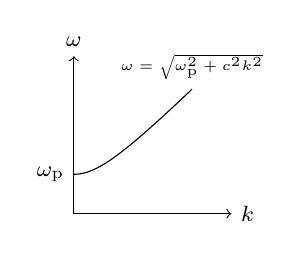
\begin{tikzpicture}[domain=0:4,scale=.5]
        \draw[->] (0,0) -- (4,0) node[anchor=west,font=\footnotesize] {$k$};
        \draw[->] (0,0) -- (0,4) node[anchor=south,font=\footnotesize] {$\omega$};
        \draw (0,1) node[anchor=east,font=\footnotesize] {$\omega_\mathrm{p}$};
        \draw[scale=1, domain = 0:3,smooth,variable=\x,black] plot ({\x},{sqrt(\x*\x+1)})
        node[above,font=\tiny] {$\omega = \sqrt{\omega_\mathrm{p}^2 + c^2 k^2}$};
\end{tikzpicture}
}
    \caption{\label{fig:dispersion}The plasma dispersion relation. We will be
        dealing with plasmas where $\omega_\mathrm{p}/\omega << 1$, so to
    first order the laser will be dispersionless. }
    \end{marginfigure}

The most important scaling behaviour of $\eta$ is with the electron's mass and
density. $\omega_p$ will scale as $\sqrt{n_e/m_e}$, so $\eta$ will scale as:
\begin{equation}
    \label{eq:etascale}
    \eta = \qty(1-\frac{n_e}{m_e}\frac{e^2}{\epsilon_0 \omega})^{1/2}
\end{equation}

Recalling that a converging lens has $d\eta/dr < 0$, the plasma
will be able to counteract diffraction in two ways: if $d
n_e/dr <0$ or $d m_e/dr >0$.

As we discussed in Section
\ref{sec:wakefield}, the first order effect of the laser will
accelerate them in the polarization plane: the quiver momentum. The electrons
will have a maximum amount of kinetic energy passing through the centre of
the laser pulse and due to relativity this corresponds to an
increase in mass. Thus, the effective mass of the electrons will have
$dm_e/dr<0$ and the plasma will act as a focusing lens.  However, in order to
use self-focusing to counteract diffraction,
the laser has to be intense enough to meaningfully change the electron mass.
This condition has been found to be $P[\si{\giga\watt}] > 17.5
\qty(\frac{\omega}{\omega_0})$ \cite{sprangle1987relativistic,sun1987self}.

There are several subtleties involved with relativistic self-focusing; chief among these is the effect
of pulse length on relativistic self-focusing. The electrons
are responding to the laser at frequency $\omega_p$, so it takes time scales on the order of $\tau_p
= \frac{1}{2\pi\omega_p}$ for the relativistic effect to build up, ie. the middle
    of the laser pulse will be `seeing' the relativistic index gradient created
    by the front of the pulse. This has two main consequences: first, long
    pulses, $\tau_\textrm{duration} > \tau_p$, are more susceptible to
    relativistic effects, and, second, the front of the pulse will be constantly
    diffracting away. Groups that primarily use relativistic self-focusing, such
    as the UT Austin group, not
    only have to choose laser pulses that are intense enough, but also that are long enough. 
    \begin{figure}[h!]
        \includegraphics[width=\textwidth]{../figures/relselffocus.pdf}
        \caption{\small A numerical simulation showing how the relativistic motion of the electrons can
            cause focusing effects\cite{genothesis}. The white curve shows the
            diffraction that would have occured in vaccuum. Self-focusing can
            extend $L_\textrm{Diffraction}$ over many Rayliegh lengths.
        }
    \end{figure}


        However, from Equation \eqref{eq:etascale} we can see that a direct
    modulation of the electron density can also achieve focusing
    effects. As long as the density goes as $dn_e/dr >0$, we have the
    appropriate condition for a converging lens. This approach is taken by
    the UC Berkeley group, where a plasma channel is used to give the
    appropriate density modulation. The plasma channel is a simple tube containing
hydrogen gas with a metal plate at each end. A voltage is applied across the
length of the tube, ionizing the gas. The gas will cool down more rapidly along
the edges of the tube, and this will give rise to an approximately parabolic
density profile of the hydrogen
gas\cite{PhysRevLett.89.185003,PhysRevE.63.015401}. It is this parabolic density
profile that
will act as the focusing lens of the plasma wave. The evolution of a laser pulse
in a plasma channel is shown in Figure \ref{fig:pchan}. 
\begin{figure}
\centering
\begin{singlespace*}
\begin{subfigure}[t]{.5\textwidth}
    \includegraphics[width=\textwidth]{../figures/plasmachannel.pdf}
    \caption{\small A simulation showing the laser spot size $r_s$ vs normalized
        propogationg distance $c\tau/L_\textrm{Raleigh}$ for (a) vacuum
        diffraction, (b) a short pulse in plasma, (c) a long pulse, intense
        enough to self-focus, and (d) a pulse guided by a plasma
    channel.\cite{sprangle1992propagation}}
\end{subfigure}
\hfill
\begin{subfigure}[t]{.45\textwidth}
    \includegraphics[width=\textwidth]{../figures/plaschan1.pdf}
    \caption{\small The input mode (a) and output mode (b)
of a laser ($I\approx 2 P_\textrm{critical}$) are nearly identical after many
diffraction lengths. Vacuum propogating over the same distance in (c).
Although the laser was firmly within the
self-focusing regime, diffraction was actually enhanced over these
distances (d)-- alluding to the difficulties in controlling self-focusing.\cite{geddes2005guiding} }
\end{subfigure}
\end{singlespace*}
\caption{Simulations showcasing the ultility of plasma-channel guiding
schemes.\label{fig:pchan}}
\end{figure}


  \section{Experimental Set-Up and State-of-the-Art}
  Now that we have discussed the underlying physics and given an overview of the
  experimental constraints  faced by modern researchers, we will highlight the
  recent results of two groups, UT
Austin and University of California Berkeley. These two groups are
on the forefront of generating  high-energy electrons through LWPA.
\subsection{UT Austin}

In 2013, the UT Austin group reported a collimated beam of \SI{2}{\giga
\electronvolt}\cite{Wang2013}. By leveraging the new petawatt laser facility at
UT Austin they were able to arrive
firmly within the experimental constraints for relativistic self-guiding.
However, due to the intense non-linear interactions involved, detailed numerical
work had to be done to find initial conditions that would produce an optimal
beam. One such example is shown in Figure
\ref{fig:propsim}\cite{Wang2013}, where by altering initial conditions such as beam
profile, startlingly different dynamics occurred. 
\begin{marginfigure}
	\includegraphics[width=\marginparwidth]{../figures/wakesimulation.pdf}
    \caption{Simulations done by the UT Austin group using the WAKE
        code showing clear features of self-focusing.\cite{Wang2013} As the
        normalized laser-intensity gets larger, the pulse is
        contracting--concentrating more of its energy over a smaller area.
        Interestingly, the self-focusing exhibits a periodic structure-- going
        through two cycles of diffraction-focusing for the super-Gaussian
    pulse.\label{fig:propsim}}
\end{marginfigure}



Numerical modeling predicted the initial conditions needed by the UT Austin to obtain high-quality mono-energetic
beams \cite{kalmykov2010numerical}. Although they were not able to produce the predicted energies,
this approach was still successful, as they were able to double the energies
of previous results\cite{PhysRevLett.113.245001}. However, their experiment
revealed some discrepancies with the numerical work, as they saw robust
self-injection with a non-uniform spot geometry.

Shown in Figure \ref{fig:experTexas} is the experimental setup for UT Austin. At
its heart, it is a high-intensity laser hitting an ionized gas. The
majority of the experiment is the diagnostics, which allow the team to determine
the energy and angular spread of the electrons.
\begin{figure}[h!]
	\includegraphics[width=\textwidth]{../figures/texasexplayout.pdf}
    \caption{\small The experimental setup of the UT Austin group.\cite{Wang2013}
        {\em This
        figure is reproduced from Nat. Commun. Vol. 4, 2013. } The laser hits
            a gas cell. It will propagate in the plasma, until the self-focusing
            process reaches a critical point, where the laser-plasma will enter
            the bubble regime. (a) Detector to measure sidescatted light
            from gas-laser interaction. (b) Schematic showing how the
            electrons are bent using a magnet-- acting like a spatial filter for
            momentum. There are tungsten posts that will cast `shadows' on the
            electron detector, allowing the source of the electrons to be
            backtracked. (c) Electron spectrum on the scintillator.
            (d) Another spectrum on the LANEX. (e)\&(f) X-ray beam
            blocker. (g) Pressure sensor on the gas cell. (h)
            Image of the laser spot-size.
        \label{fig:experTexas} }
    
\end{figure}

The UT Austin group is now developing strategies to increase the
energy of the electron beam. Further progress can only be made with an increased
understanding of the dynamics of the laser-plasma acceleration, specifically
relativistic self-focusing and self-injection, and to that end
they have developed novel imaging techniques that,
taken together with numerical simulations, form a powerful platform for moving
forward.\cite{dong2010laboratory,li2014single}

\subsection{UC Berkeley}
In 2014, the Berkeley group reported a collimated electron beam with peak
energy of \SI{4.2}{\giga \electronvolt}. They achieved this through a slightly
different experimental philosophy than the UT Austin group.
\begin{marginfigure}[-100pt]
    \includegraphics[width=\marginparwidth]{../figures/esaenergy.pdf}
    \caption{The energy spectrum for the recent Berkeley result.}
\end{marginfigure}
By using lower intensity
short-duration lasers, they are able to use a plasma-channel guide that may be
damaged by higher-intensity lasers. Although
relativistic self-focusing is still required to achieve the high-intensities
needed for the bubble regime, the plasma-channel does the majority of the work
in preventing laser diffraction. Their use of a lower intensity laser has two
main benefits. First, they gain on energy conversion efficiency.
\begin{marginfigure}
	\includegraphics[width=\marginparwidth]{../figures/esareycapfield.pdf}
    \caption{Evolution of the peak normalized intensity of the laser pulse,
    ($a_0(z)$ done using a particle-in-cell simulation for a top-hat laser pulse
    with energy 16 J, through a 9 \si{cm} plasma waveguide. {\em From Leemans
et. al. 2014 \cite{PhysRevLett.113.245002}}\label{fig:esasim}}
\end{marginfigure}
As though the acceleration gradients are smaller, they are able to guide them
over larger distances. Second, because the laser is lower intensity, the dynamics
of self-focusing and non-linear laser-plasma interactions are less
pronounced, simplifying the dynamics of the laser propogation. However,
they will ultimately be limited by the pump-depletion length, as the laser
simply has less energy than the UT Austin petawatt laser.

\section{Conclusion}
In this review, we have discussed the basic physics processes of LWPA and
summarized two approaches for electron acceleration:
the high-intensity, relativistically guiding approach used by UT Austin; and the
low-intensity, plasma-channel guided approach used by Berkeley.

For further
progress to be made in the field there needs to be a better understanding of
the laser-plasma interaction. The new imaging
techniques at UT Austin, which allow in vivo imaging of the evolution
of the laser and plasmon, is a key contribution as it allows direct comparison to numerical
simulations. This is invaluable in efforts to harness the phenomena of
self-injection and self-focusing for LWPA technology and an exciting
opportunity to develop and refine numerical approaches. 

With the current record of \SI{4.2}{\giga\electronvolt}, LWPA
technology is within striking distance of current linear accelerator technology,
and with the dynamic progress being made across the entire field, it is clear
that LWPA will soon be able to make a broad impact in the scientific
community. The raw power exists to accelerate
electrons to high GeV energies, all we need to do is control it.
\bibliography{../rep.bib}
\end{document}

